\documentclass[a4paper,14pt]{extarticle}

\usepackage{ucs}                                                                                                                   
\usepackage[utf8x]{inputenc}                                                                                                       
\usepackage[english,russian]{babel}
\usepackage[T2A]{fontenc}
\usepackage{extsizes}
\usepackage{tempora}
\usepackage[left=30mm, top=20mm, right=15mm, bottom=20mm, headheight=5pt]{geometry}
\usepackage{fancyhdr}
\usepackage{titling}
\usepackage{titlesec}
\usepackage{textcase}
\usepackage{indentfirst}
\usepackage{graphicx}
\usepackage{float}
\usepackage[labelsep=endash]{caption}
\usepackage{listings}
\usepackage{color}
\usepackage{enumitem}
\usepackage[font=normalsize]{subfig}

\graphicspath{ {./images/} }

\newcommand{\mylabnumber}{1}
\newcommand{\mylabtitle}{Встроенные типы данных в C\#. Массивы. Строки. Регулярные выражения}
\newcommand{\mysubject}{Платформа .NET}
\newcommand{\mylecturer}{ст. преп. Забаштанский А.К.}

\renewcommand{\baselinestretch}{1.25} % Sets basic line stretch
\renewcommand{\headrulewidth}{0pt} % Remove horizontal line below header in fancyhdr

\addto\captionsrussian{
    \renewcommand{\figurename}{Рисунок} % Set a default picture caption
    \renewcommand{\tablename}{Таблица} % Set a default table caption
}

\captionsetup[table]{singlelinecheck=false} % To make a table caption appear left-aligned

\pagestyle{fancy}
\lhead{} \rhead{} \cfoot{} % Setting empty headers
\chead{\thepage} % Sets central header page numbering

\setlength{\parindent}{1.25cm}
\setlength{\parskip}{8pt}

 % Format section style and indentations
\titleformat{\section}[hang]
    {\large \centering \bfseries}
    {\thesection}
    {0.5em}
    {\MakeTextUppercase}
\titlespacing{\section}{\parindent}{1em}{0em}

% Format subsection style and indentations
\titleformat{\subsection}[hang]
    {\bfseries}
    {\thesubsection}
    {0.5em}{}
\titlespacing{\subsection}{\parindent}{1em}{0em}

% Format subsubsection style and indentations
\titleformat{\subsubsection}[hang]
    {\normalfont}
    {\thesubsubsection}
    {0.5em}
    {}
\titlespacing{\subsubsection}{\parindent}{1em}{0em}

% Format enumerate style with "enumitem" package
\setlist[enumerate]{
    wide=\parindent,
    leftmargin=0pt,
    topsep=0pt,
    itemsep=0pt,
    partopsep=0pt,
    parsep=0pt
}

% Format itemize style with "enumitem" package
\setlist[itemize]{
    wide=\parindent,
    leftmargin=0pt,
    topsep=0pt,
    itemsep=0pt,
    partopsep=0pt,
    parsep=0pt
}

\begin{document}

    \lstset{ % "listings package configuration"
        basicstyle=\footnotesize\ttfamily,
        numbersep=5pt,
        tabsize=4,
        gobble=8,
        extendedchars=\true,
        keepspaces=\true,
        numbers=left,
        keywordstyle=\color{cyan},
        stringstyle=\color{red}\ttfamily,
        commentstyle=\color{green},
        showstringspaces=\false
    }

    \begin{titlepage}
        
        \thispagestyle{empty}
        
        \begin{center}
            
            Министерство науки и высшего образования Российской Федерации \\
            Севастопольский государственный университет \\
            Кафедра ИС
            
            \vfill
            \large{
                Отчет \\
                по лабораторной работе №\mylabnumber \\
                "\mylabtitle" \\
                по дисциплине \\
                \MakeTextUppercase{\mysubject}
            }

        \end{center}

        \vspace{1cm}

        \noindent\hspace{7.5cm} Выполнил студент группы ИС/б-22о \\
        \null\hspace{7.5cm} Горбенко К. Н. \\
        \null\hspace{7.5cm} Проверил \\
        \null\hspace{7.5cm} \mylecturer

        \vfill

        \begin{center}
            Севастополь \\
            2019
        \end{center}

    \end{titlepage}

    % ############################################################################
    % ------------------------------ Document start ------------------------------
    % ############################################################################

    \section{Цель работы}

    \begin{itemize}
        
        \item изучить классификацию типов данных и отличительные 
              особенности синтаксических конструкций языка C\# от C++;

        \item изучить базовые типы: Array, String, StringBuilder, а также
              средства стандартного ввода/вывода и возможности форматирования
              вывода;

        \item получить понятие о регулярных выражениях и их применении
              для поиска, замены и разбиения текста на синтаксические лексемы.

    \end{itemize}

    \section{Задание к лабораторной работе}

    Для \textbf{варианта № 3} заданы следующие задания:
    
    \begin{enumerate}
        
        \item Проработать примеры программ 1-8, данные в теоретических сведениях.
              Создать на их основе программы. Получить результаты работы программ
              и уметь их объяснить. Внести их в отчет по работе с комментариями.

        \item Найти номер столбца двухмерного массива целых чисел, для которого
              среднеарифметическое его элементов максимально.
              
        \item Создать программу, которая будет вводить строку в переменную String.
              Найти в ней те слова, которые начинаются и заканчиваются одной и 
              той же буквой.

        \item Задан текст. Определить, является ли он текстом на английском языке.

    \end{enumerate}
    
    \section{Ход работы}

    \subsection{Примеры программ на C\#}

    \subsubsection{Пример № 1}

    Результат работы программы № 1:

    \begin{figure}[H]
        \centering
        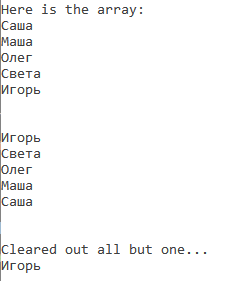
\includegraphics[width=.4\textwidth]{Example1}
        \caption{Результат работы программы из примера № 1}
    \end{figure}

    В примере № 1 демонстрируются статические методы Reverse и Clear
    класса Array.

    \subsubsection{Пример № 2}

    Результат работы программы № 2:

    \begin{figure}[H]
        \centering
        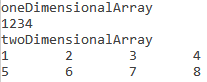
\includegraphics[width=.4\textwidth]{Example2}
        \caption{Результат работы программы из примера № 2}
    \end{figure}

    В программе демонстрируется возможность передать любой массив
    в функцию с помощью абстрактного класса Array. При этом индексирование
    массива происходит с помощью методов GetValue.

    \subsubsection{Пример № 3}

    Результат работы программы № 3:

    \begin{figure}[H]
        \centering
        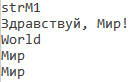
\includegraphics[width=.4\textwidth]{Example3}
        \caption{Результат работы программы из примера № 3}
    \end{figure}

    В данной программе исследуется тип данных char и возможность
    перехода от массива символов к строке и наоборот. Для перевода
    строки в массив символов используется метод класса String ToCharArray.
    Для обратной операции используется цикл for. Однако лучше это сделать 
    с помощью конструктора класса String, принимающего массив символов.

    \subsubsection{Пример № 4}

    Результат работы программы № 4:

    \begin{figure}[H]
        \centering
        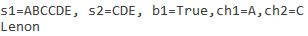
\includegraphics[width=.4\textwidth]{Example4}
        \caption{Результат работы программы из примера № 4}
    \end{figure}

    В данной программе демонстрируется класс StringBuilder, который
    используется для увеличения производительности при работе со строками.
    Основные методы: Append, Remove, Insert.

    \subsubsection{Примеры № 5, № 6, № 7}

    В программах № 5, № 6 и № 7 исследуются способы использования регулярных выражений
    для поиска соответствий в строке. Для данной цели могут использоваться 
    статические методы Matches и Match, принимающие как строку, так и 
    шаблон, а также те же методы класса Regex, инициализированного с 
    шаблоном в конструкторе.

    \subsubsection{Пример № 8}

    \begin{figure}[H]
        \centering
        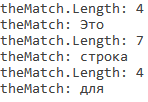
\includegraphics[width=.4\textwidth]{Example8}
        \caption{Результат работы программы из примера № 4}
    \end{figure}

    В данной программе в шаблон регулярного выражения включаются именованные группы.

    \subsection{Индивидуальное задание для работы над массивами}

    Была написана следующая программа:

    \begin{lstlisting}[language={[Sharp]C}]
        public static class ArrayOperations
        {
            public static int GetMaximalAverageColumn(int[,] matrix)
            {
                if (matrix == null) 
                    throw new ArgumentNullException($"{nameof(matrix)} instance was null");

                var columnsAverages = matrix
                                        .GetColumns()
                                        .Select(x => x.Average())
                                        .ToArray();

                return Array.IndexOf(columnsAverages, columnsAverages.Max());
            }

            public static void PrintMatrix(int[,] matrix)
            {
                if (matrix == null) 
                    throw new ArgumentNullException($"{nameof(matrix)} instance was null");

                for (var i = 0; i < matrix.GetLength(0); i++)
                {
                    for (var j = 0; j < matrix.GetLength(1); j++)
                        Console.Write($"{matrix[i, j]} ");

                    Console.WriteLine();
                }
            }
        }

        public static class ExtensionMethods
        {
            public static IEnumerable<int[]> GetColumns(this int[,] array)
            {
                if (array == null) 
                    throw new ArgumentNullException($"{nameof(array)} instance was null");

                for (var j = 0; j < array.GetLength(1); j++)
                {
                    var column = new int[array.GetLength(0)];
                    
                    for (var i = 0; i < array.GetLength(0); i++)
                        column[i] = array[i, j];

                    yield return column;
                }
            }
        }

        public class Program
        {
            public static void CheckArrays()
            {
                WriteLine("Checking arrays task");

                const int M = 5;
                const int N = 10;
                var matrix = new int[M, N];
                var random = new Random();

                for (var i = 0; i < matrix.GetLength(0); i++)
                    for (var j = 0; j < matrix.GetLength(1); j++)
                        matrix[i, j] = random.Next(100);

                ArrayOperations.PrintMatrix(matrix);

                WriteLine("\nAverages:\n");
                foreach (var item in matrix.GetColumns().Select(x => x.Average()))
                    Write($"{item} ");

                WriteLine($"\nColumn with maximal average: {ArrayOperations.GetMaximalAverageColumn(matrix)}");
            }
        }
    \end{lstlisting}

    Результат работы программы:

    \begin{figure}[H]
        \centering
        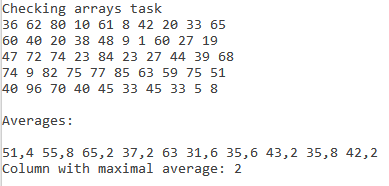
\includegraphics[width=.4\textwidth]{Arrays}
        \caption{Результат работы программы с операциями над массивами}
    \end{figure}

    В данной программе активно используется библиотека System.Linq для операций
    над коллекциями. Также был написан extension-метод для извлечения столбцов
    матрицы. Для определения позиции с наибольшим средним столбцом в строке
    использовался статический метод IndexOf класса Array.

    \subsection{Индивидуальное задание для работы над строками}

    Была написана следующая программа:

    \begin{lstlisting}[language={[Sharp]C}]
        public static class StringOperations
        {
            public static IEnumerable<string> GetWordsStartingAndEndingTheSameLetter(string line)
                => line.Split(" ").Where(x => x.First() == x.Last());
        }

        public class Program
        {
            public static void CheckStrings()
            {
                WriteLine("Checking strings task");

                WriteLine("Enter your string:");
                var str = ReadLine();

                WriteLine("Words starting and ending with the same letter:");
                foreach (var word in StringOperations.GetWordsStartingAndEndingTheSameLetter(str))
                    Write($"{word} ");
            }
        }
    \end{lstlisting}

    Результат работы программы:

    \begin{figure}[H]
        \centering
        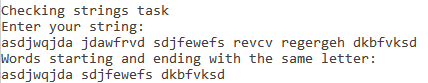
\includegraphics[width=.4\textwidth]{Strings}
        \caption{Результат работы программы с операциями над строками}
    \end{figure}

    В данной программе используется метод Split класса String для разделения
    строки на подстроки, а также библиотека System.Linq для фильтрации 
    полученной коллекции. Условием для фильтра является равенство результатов
    выполнения методов First и Last класса String, возвращающих соответственно
    первый и последний символы строки.

    \subsection{Индивидуальное задание для работы с регулярными выражениями}

    Была написана следующая программа:

    \begin{lstlisting}[language={[Sharp]C}]
        public static class RegexOperations
        {
            private static string englishRegexTemplate = @"^[A-Za-z0-9 .,!?:;()]+$";

            public static bool IsInEnglish(string test)
                => Regex.IsMatch(test, englishRegexTemplate);
        }

        public class Program
        {
            public static void CheckRegexes()
            {
                WriteLine("Checking regex task");

                var englishText    = "A text in English with some punctuation marks:.,;!?()";
                var notEnglishText = "Текст не на английском. Всякие знаки препинания:.?,!";

                WriteLine(englishText);
                WriteLine(RegexOperations.IsInEnglish(englishText));

                WriteLine(notEnglishText);
                WriteLine(RegexOperations.IsInEnglish(notEnglishText));
            }
        }
    \end{lstlisting}

    Результат работы программы:

    \begin{figure}[H]
        \centering
        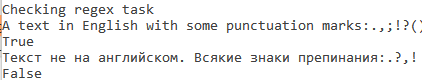
\includegraphics[width=.4\textwidth]{Regexes}
        \caption{Результат работы программы с операциями над регулярными выражениями}
    \end{figure}

    В данной программе создан класс, полем которого является шаблон регулярного
    выражения, осуществляющего проверку того, что все встреченные в строке символы
    являются либо буквами английскго алфавита, либо арабскими цифрами, либо пробелами,
    либо знаками пунктуации. 

    Для вызова регулярного выражения использовался статический метод Regex.IsMatch,
    который принимает как входную строку, так и сам шаблон регулярного выражения.

    \section{Вывод}

    В ходе лабораторной работы были изучены массивы, строки и регулярные выражения
    языка C\#, а также встроенные средства для работы с ними. 
    
    Все массивы в среде .NET являются наследниками абстрактного класса Array,
    что позволяет передавать в одну и ту же функцию любой массив. Кроме того,
    класс Array предоставляет множество статических методов и методов экземпляра
    для эффективной работы с массивами.

    Строки в платформе .NET являются неизменяемыми, что приводит к просадкам в
    производительности при выполении множества операций над ними. Для избежания
    проблем с производительность в таких случаях используют класс StringBuilder.
    Класс String также содержит множество методов для работы со строками.

    Регулярные выражения - мощный инструмент для работы со строками. Они позволяют
    проверять строку на соответствие шаблону и производить поиск подстрок в строке.
    Соответствующие операции обычными методами более трудозатратны.

\end{document}